\chapter{general presentation of the test network}


\section{Goals}

The foal of the project was to build a test network for the Mesh Extenders. 
We want to have Mesh Extenders at different places in a building. The Mesh extenders are communicating together using UHF (they need to far enough from each other or have their Wi-Fi range limited by any way). Each Mesh extender is connected to a phone by Wi-Fi.

The test network is built around this basic setup. We want to be able to remotely supervise and control each site.
To do that we are going to built a test network with:
\begin{itemize}
	\item a software part using c programs
	\item a hardware part using small linux routers
\end{itemize}



\section{Components}

As previously said, the test network is made of a software and a hardware part.

\subsection{Hardware components}

First, for this test network, we will obviously need Mesh Extenders:
\begin{figure}[H]
\begin{center}
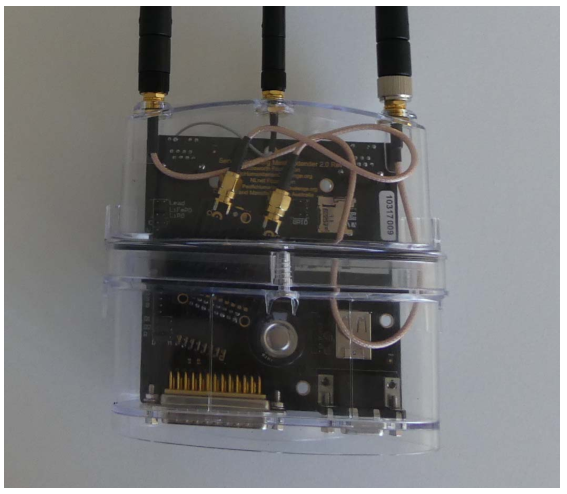
\includegraphics[width=8cm]{image/meshextender.png}%
\caption{Mesh Extender}%
\label{figure:ME}%-
\end{center}
\end{figure}


In this project we are also using small linux routers to built the network we will use to supervise the Mesh Extenders.

The small router we have chose to use are: the GL-AR150 and GL-AR750.

\begin{figure}[H]
\centering
\begin{subfigure}{.5\textwidth}
  \centering
	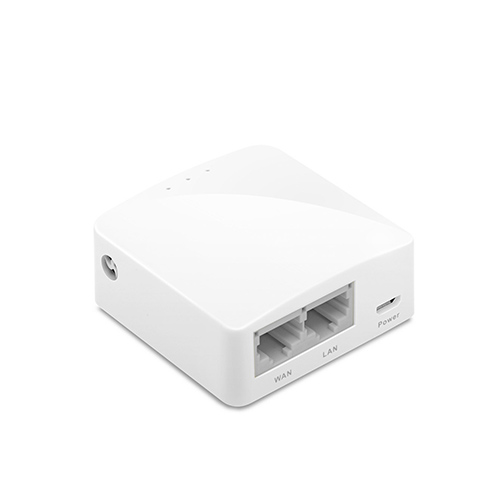
\includegraphics[width=8cm]{image/AR150.jpg}%
	\caption{GL-AR150}%
	\label{figure:AR150}%-
\end{subfigure}%
\begin{subfigure}{.5\textwidth}
  \centering
  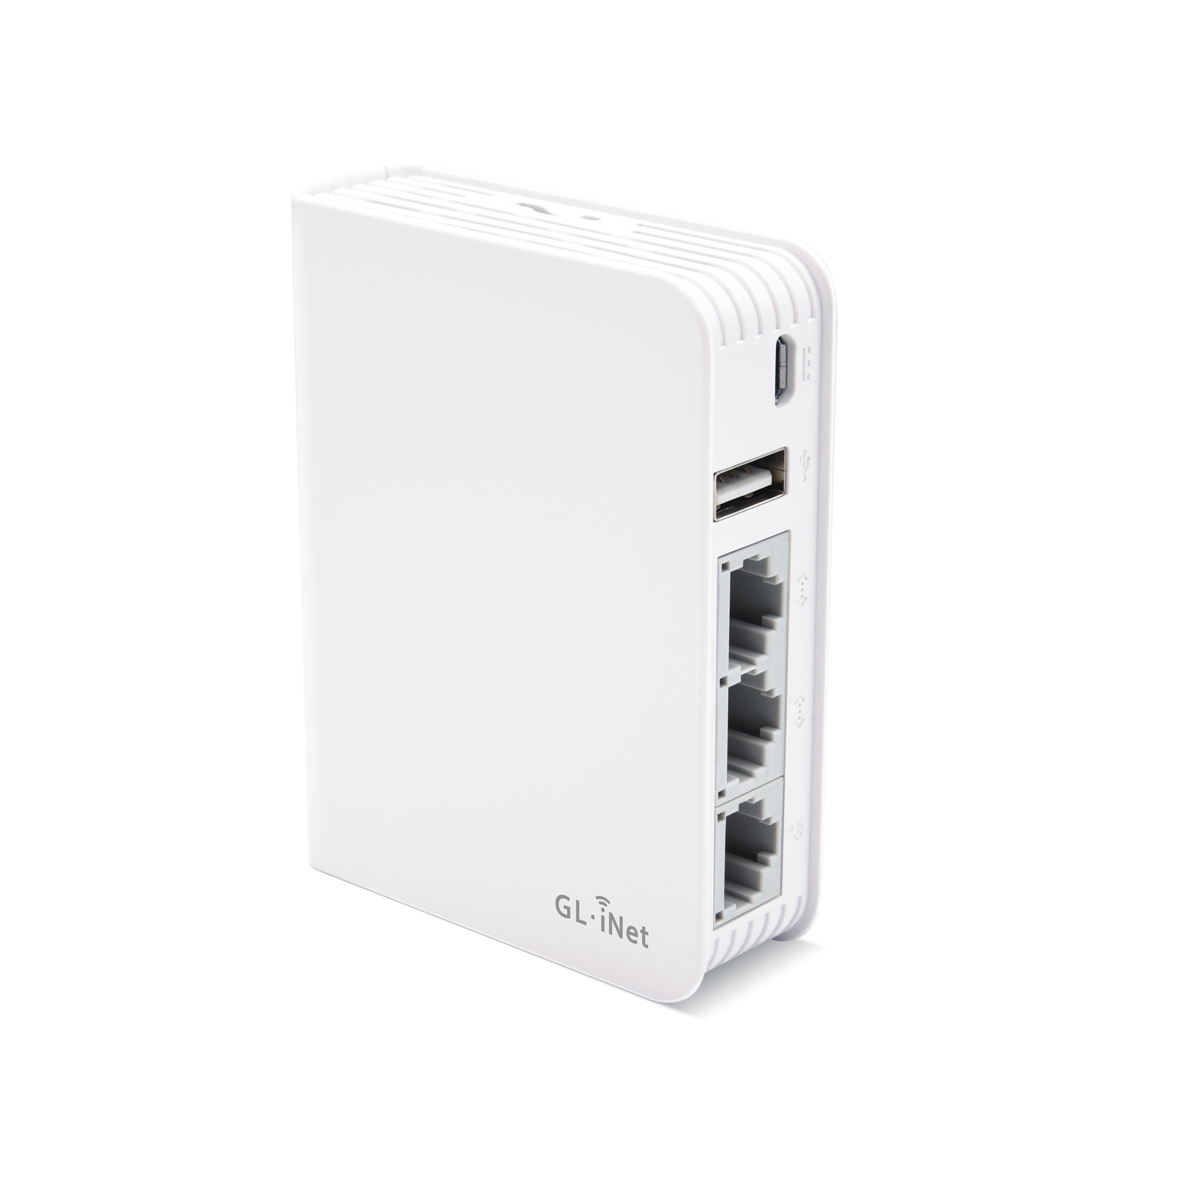
\includegraphics[width=8cm]{image/AR750.jpg}%
	\caption{GL-AR750}%
	\label{figure:AR750}%-
\end{subfigure}
\caption{Routers used for the testbed}
\label{fig:routers}
\end{figure}


These two routers are great for the test network. Indeed, they are small, affordable and we have a lot of freedom since their OS is based on a Linux kernel (the OS used for the Mesh extenders can also be put inside these routers).
The only issue we can have is the fact they do not have a lot of USB port and also no UHF radio. Therefore we need other devices:
\begin{figure}[H]
\centering
\begin{subfigure}{.5\textwidth}
  \centering
	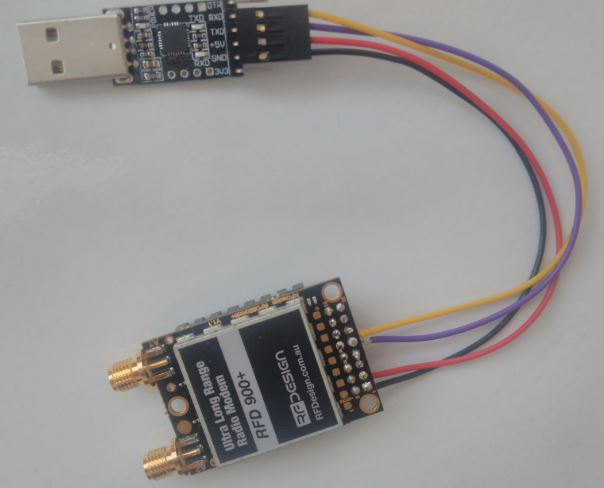
\includegraphics[width=8cm]{image/rfd900.jpg}%
	\caption{RFD900 with a serial to USB adapter}%
	\label{figure:RFD900}%-
\end{subfigure}%
\begin{subfigure}{.5\textwidth}
  \centering
  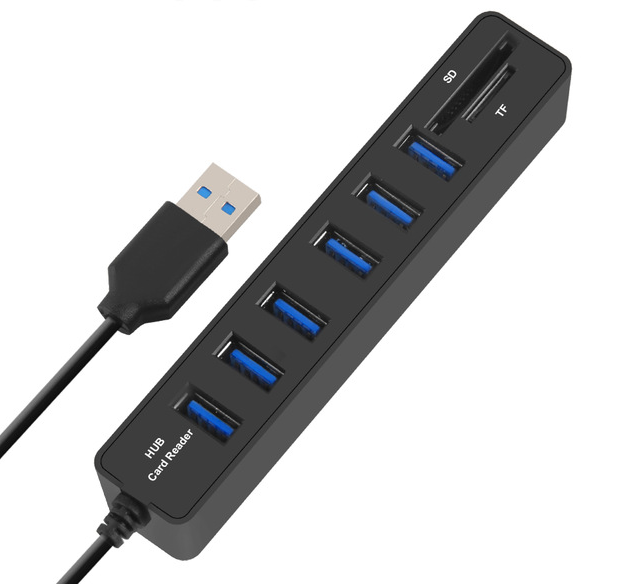
\includegraphics[width=8cm]{image/usbhub.jpg}%
	\caption{USB hub}%
	\label{figure:UsbHub}%-
\end{subfigure}
\caption{Other devices needed}
\label{fig:devices}
\end{figure}

To monitor the UHF packets of the Mesh Extenders, we need a RFD900+. Since the RFD900+ has a serial interface (pins), we need to create an adapter to plug it using USB.
We are using a USB hub to increase the number of USB ports on the router.

We now have all the needed hardware.



\subsection{software}

In this project, we are going to use c programs to remotely supervise the Mesh Extenders.
C language was chosen because:
\begin{itemize}
	\item it is a light and efficient language (which is great since our routers don't have a lot of power or memory)
	\item In the Serval project most of the coding was made in c. We can easily integrate other part of the serval project inside the test network.
\end{itemize}


I have decide to create a TCP client-server system composed of 3 files:
\begin{itemize}
	\item server.c which will be on the small routers
	\item client\_shell.c and client.c which will be on the computer used to supervise
\end{itemize}

I will explain what each file does in the next section.


A TCP client-server was not the only solution. However, I still opted for it because:
\begin{itemize}
	\item I was more used to code TCP server and client than other solutions. Therefore I will be faster using this solution.
	\item The libraries for TCP are quite old and should work on most devices.
\end{itemize}



\section{Big picture}

We will now take a look at how the network and software work.


\subsection{Big picture of the network}
%BIG  picture of the network





\subsection{Big picture of the software}



The software part corresponds to the communication between a few programs:
\begin{itemize}
	\item the client\_shell and the client
	\item the client and the server
	\item the server and the RFD900+
\end{itemize}

For the communication between the server and the RFD900+, we use the driver in c developed by Paul. This part use the code of the lbard git repository.


\subsubsection{client to server communication}

The communication between the client and the server is very basic. Most of the time the client is only receiving packet from the server and display them on the computer.

But the client can also send a few message to the server. This messages allow the client to close the communication with the server. Later they will also allow the client to change what is supervised.

\begin{figure}[H]
\begin{center}
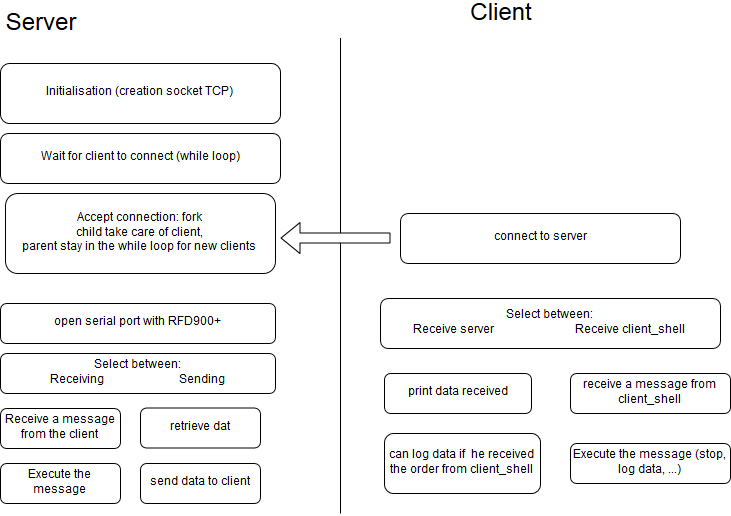
\includegraphics[width=\textwidth]{image/clientServer.png}%
\caption{Client and server communication}%
\label{figure:CS}%-
\end{center}
\end{figure}





\subsubsection{client\_shell and client interactions}

The client\_shell is a shell-like interface that gives access to all the available functionalities.
It can:
\begin{itemize}
	\item find the available servers using a file containing the hostnames of servers
	\item launch a client
	\item communicate with the client to send different orders such as
		\subitem "`STOP"' to close the connection
		\subitem "`LOG Filename"' to start logging the data
  \item keep a list of all the current client created
	\end{itemize}




\begin{figure}[H]
\begin{center}
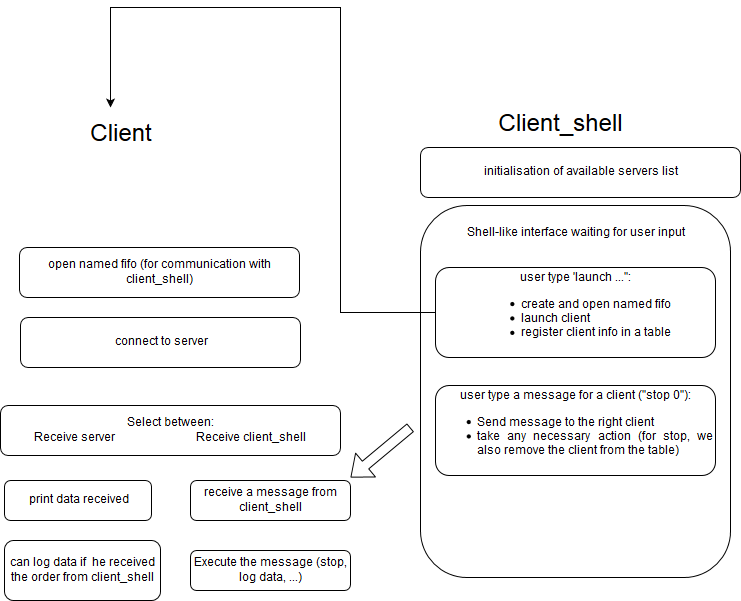
\includegraphics[width=\textwidth]{image/clientshellClient.png}%
\caption{Client and Client\_shell interaction}%
\label{figure:CSC}%-
\end{center}
\end{figure}

